\documentclass[12pt]{article}

\usepackage{sbc-template}
\usepackage{graphicx,url}
\usepackage{xcolor}
\usepackage{array}
\usepackage[utf8]{inputenc}
\usepackage[brazil]{babel}
\usepackage{indentfirst}
%\usepackage[latin1]{inputenc}  

     
\sloppy

\title{Algoritmos de validação da confiança em sistemas de automação inteligente}

\author{Gabriel Egídio Santos Beloni\inst{1}, Gabriel Evangelista Massara\inst{2}}


\address{ICEI -- Pontifícia Universidade Católica
  (PUC-MG)\\
  CEP 91.501-970 -- Belo Horizonte -- MG -- Brasil
}

\begin{document} 

\maketitle

\section{Introdução}
\subsection{Contextualização}

A aplicação da inteligência artificial em sistemas de automação inteligente tem ampliado a capacidade de softwares executarem tarefas, tomarem decisões operacionais e apoiarem processos que antes dependiam integralmente de intervenção humana. Com a popularização de modelos de linguagem, agentes autônomos, fluxos automatizados e integrações entre sistemas, tornou-se possível construir soluções capazes de interpretar entradas variáveis, acionar ferramentas externas e adaptar seu comportamento a diferentes contextos de uso. Esse avanço, entretanto, também aumenta a responsabilidade sobre a forma como essas soluções são projetadas, avaliadas e colocadas em operação.

Nesse cenário, a confiança deixa de ser apenas uma percepção subjetiva do usuário e passa a depender de mecanismos objetivos de validação. Um sistema de automação inteligente precisa demonstrar que suas ações são consistentes, rastreáveis, autorizadas e compatíveis com as regras do domínio em que atua. Quando uma automação executa comandos sem validação adequada, utiliza dados incorretos ou toma decisões sem critérios verificáveis, ela pode gerar falhas operacionais, prejuízos financeiros, exposição de informações sensíveis e perda de credibilidade. Por isso, investigar algoritmos capazes de validar a confiança nesses sistemas é essencial para garantir que a automação não apenas funcione, mas funcione dentro de limites seguros, auditáveis e previsíveis.

\subsection{Justificativa}

A escolha deste tema decorre da necessidade crescente de desenvolver sistemas de automação inteligente que sejam capazes de operar com maior autonomia sem comprometer a segurança, a confiabilidade e o controle humano sobre os processos automatizados. O desafio atual não está somente em criar mecanismos que executem tarefas de forma automática, mas em definir critérios que permitam verificar se uma ação sugerida ou realizada por um sistema inteligente pode ser considerada confiável antes, durante e depois de sua execução.

Em aplicações reais, sistemas de automação baseados em inteligência artificial lidam com dados dinâmicos, regras de negócio variáveis e diferentes níveis de incerteza. Essa característica torna indispensável a existência de algoritmos de validação que considerem fatores como coerência da resposta, origem dos dados utilizados, permissões do usuário, histórico de ações, explicabilidade, nível de risco e conformidade com regras previamente definidas. Sem esse tipo de validação, a automação pode produzir resultados aparentemente corretos, mas inadequados ao contexto, inseguros ou impossíveis de justificar tecnicamente.

Dessa forma, estudar algoritmos de validação da confiança contribui para a construção de soluções mais robustas, transparentes e aplicáveis ao mundo real. A pesquisa também se justifica pela necessidade de aproximar os avanços recentes da inteligência artificial de práticas de engenharia de software que favoreçam manutenção, auditoria, governança e redução de riscos. Ao propor ou analisar mecanismos de validação, torna-se possível melhorar a qualidade dos sistemas de automação inteligente e aumentar a segurança de sua adoção em ambientes corporativos, acadêmicos e operacionais.

\subsection{Motivação}

A motivação para esta pesquisa está relacionada ao crescimento de ferramentas e plataformas que permitem criar automações inteligentes com pouco esforço técnico, mas que nem sempre oferecem mecanismos suficientes para verificar a confiabilidade das ações executadas. Em muitos casos, agentes e fluxos automatizados são colocados em uso com base apenas na expectativa de que a inteligência artificial produzirá uma resposta adequada, sem que existam critérios claros para validar a decisão tomada, registrar sua justificativa ou impedir comportamentos indevidos.

Esse cenário evidencia a importância de investigar formas algorítmicas de medir, validar e controlar a confiança em sistemas de automação inteligente. A partir dessa perspectiva, torna-se possível compreender quais características devem ser observadas para que uma automação seja considerada segura e confiável, bem como quais mecanismos podem ser aplicados para reduzir erros, limitar ações de risco e manter o ser humano no controle das decisões mais sensíveis. Assim, a pesquisa busca contribuir para o desenvolvimento de sistemas que não sejam apenas automatizados, mas também verificáveis, controláveis e adequados às exigências práticas de uso.


\section{Referencial Teórico}

O referencial teórico deste trabalho tem como finalidade reunir os conceitos necessários para compreender a validação da confiança em sistemas de automação inteligente. A discussão parte da evolução da automação tradicional para arquiteturas capazes de interpretar dados, reconhecer padrões, adaptar-se ao ambiente e executar ações com diferentes graus de autonomia. Em seguida, são analisadas as dimensões que sustentam a confiança nesses sistemas: qualidade dos dados, adequação ao contexto, segurança, controle, rastreabilidade e validação algorítmica da decisão. Dessa forma, o referencial não trata a confiança apenas como uma percepção subjetiva do usuário, mas como uma propriedade técnica, operacional e sociotécnica que precisa ser verificada ao longo de todo o ciclo de funcionamento da automação.

\subsection{Automação inteligente}

A automação tradicional pode ser compreendida como a execução programada de tarefas a partir de regras previamente definidas. Nesse modelo, o sistema tende a responder a eventos conhecidos por meio de comandos fixos, com pouca ou nenhuma capacidade de adaptação. A automação inteligente, por sua vez, amplia esse modelo ao incorporar técnicas de inteligência artificial, aprendizado de máquina, sensores, dispositivos conectados e mecanismos de análise de dados. Com isso, o sistema deixa de apenas executar rotinas repetitivas e passa a perceber variáveis do ambiente, interpretar entradas incertas, comparar padrões e apoiar decisões operacionais.

Essa mudança é especialmente relevante em ambientes associados à Internet das Coisas (IoT), nos quais dispositivos físicos e digitais passam a interagir continuamente. Em tais cenários, sensores, atuadores, aplicações e serviços em rede produzem grande quantidade de dados e permitem que decisões sejam tomadas com menor intervenção humana. No artigo \textit{Trust Management in the Internet of Things: A Survey}, Mohammed A. Ferrag, Leandros Maglaras e Helge Janicke \cite{ferrag2019} apresentam um levantamento sobre modelos de gerenciamento de confiança em ambientes de Internet das Coisas. O trabalho analisa abordagens baseadas em reputação, criptografia e aprendizado de máquina, destacando desafios como escalabilidade, heterogeneidade dos dispositivos e vulnerabilidades de segurança. Essa contribuição é relevante para a automação inteligente porque demonstra que sistemas conectados não podem depender apenas da execução automática de comandos, mas precisam de mecanismos capazes de avaliar se as interações entre dispositivos, usuários e serviços são confiáveis.

No artigo \textit{Estudo da inteligência artificial aplicada em Internet das Coisas, voltada na automação residencial}, Welliton Sousa da Cunha \cite{cunha2018} discute a integração entre inteligência artificial e Internet das Coisas como uma evolução da automação convencional. A chamada domótica inteligente não se limita a ligar ou desligar dispositivos a partir de comandos fixos; ela busca interpretar o comportamento dos usuários, aprender hábitos e adaptar respostas conforme o contexto. Esse exemplo demonstra que a automação inteligente é caracterizada por um ciclo contínuo de percepção, inferência e ação. Quanto mais esse ciclo se torna autônomo, maior passa a ser a necessidade de validar se a ação sugerida ou executada pelo sistema pode ser considerada confiável.

Nesse sentido, a automação inteligente pode ser compreendida como uma arquitetura composta por quatro etapas principais: coleta de dados, interpretação algorítmica, decisão e execução. A validação da confiança deve atuar de forma transversal a essas etapas, verificando se os dados utilizados são adequados, se a inferência produzida é coerente, se o contexto permite a ação e se existem permissões suficientes para sua execução. Portanto, a inteligência de um sistema automatizado não deve ser avaliada somente por sua capacidade de agir, mas também por sua capacidade de justificar, limitar e controlar suas próprias ações.

\begin{figure}[htbp]
    \centering
    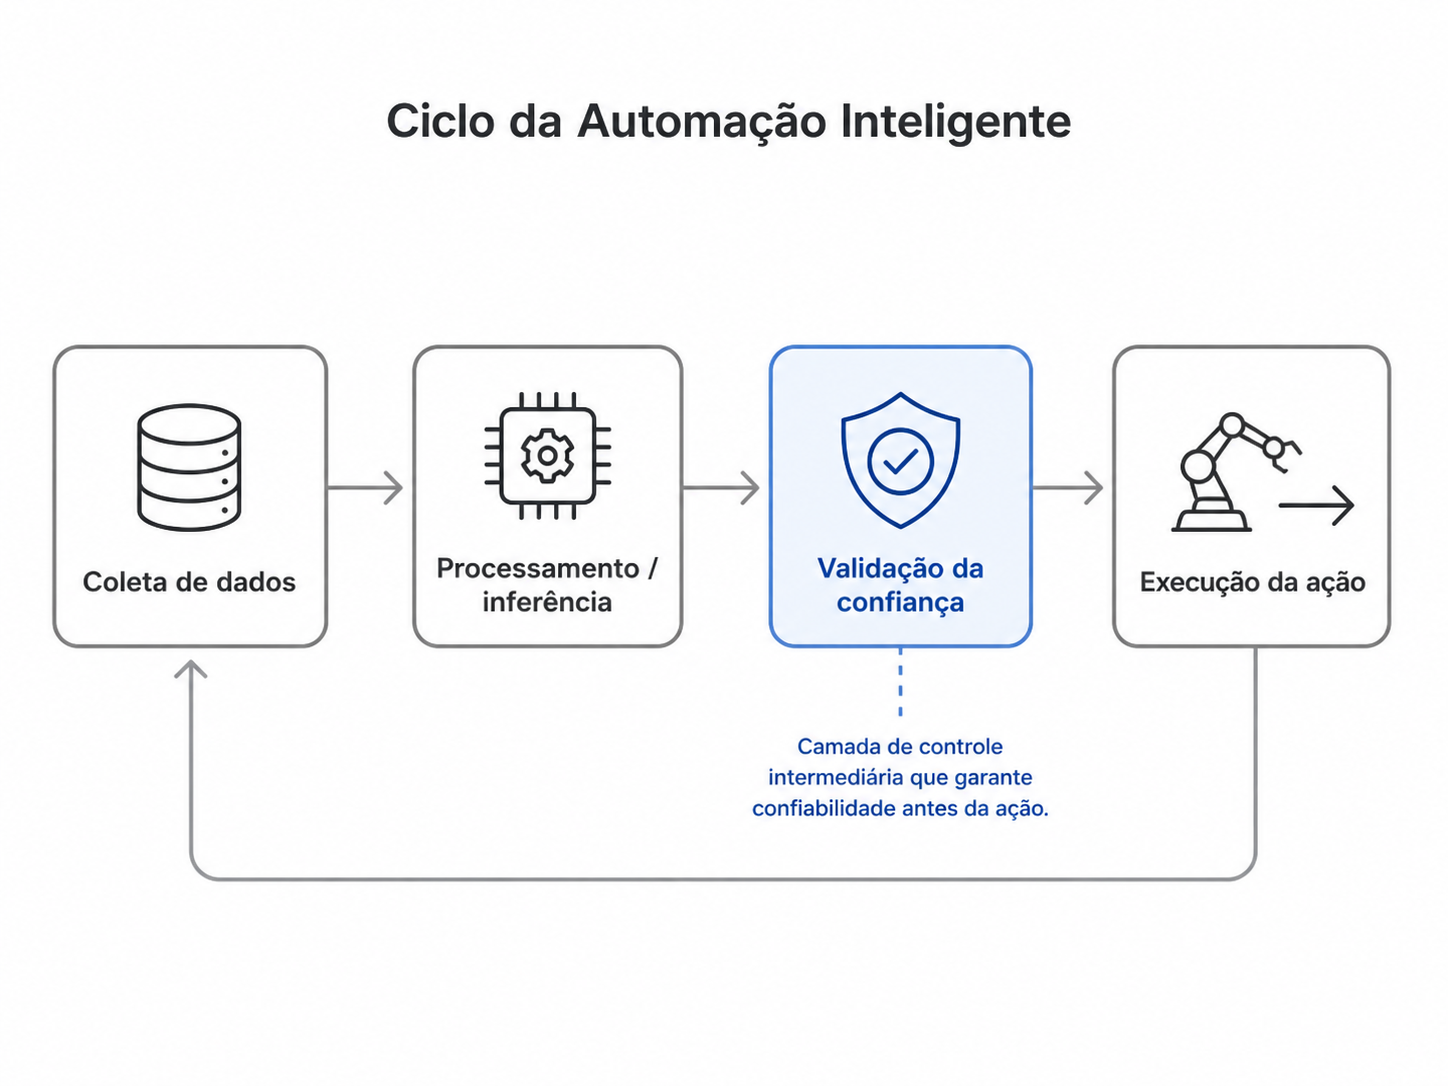
\includegraphics[width=0.5\linewidth]{img/cicloAutomacao.png}
    \caption{Ciclo da Automação Inteligente}
    \label{fig:ciclo-automacao}
\end{figure}

\subsection{Confiança em sistemas automatizados}

A confiança em sistemas automatizados não deve ser reduzida à ideia de que o sistema apresenta bom desempenho estatístico ou alta taxa de acerto. Embora métricas como precisão, revocação, taxa de erro e estabilidade sejam importantes, elas não são suficientes para determinar se uma decisão automatizada deve ser aceita em um ambiente real. Um sistema pode produzir uma resposta tecnicamente plausível e, ainda assim, ser inadequado por utilizar dados desatualizados, violar uma regra de negócio, agir sem autorização, apresentar risco excessivo ou não oferecer rastreabilidade suficiente para auditoria.

No contexto deste trabalho, a confiança é tratada como uma propriedade multidimensional. Isso significa que uma decisão automatizada é confiável quando atende simultaneamente a critérios de coerência técnica, segurança, legitimidade operacional, adequação contextual e possibilidade de verificação posterior. A confiança, portanto, não é apenas uma característica do algoritmo de inteligência artificial, mas o resultado da interação entre algoritmo, dados, infraestrutura, permissões, usuários e ambiente de execução.

A literatura de segurança em IoT reforça essa visão. No artigo \textit{Trust Management in the Internet of Things: A Survey}, Ferrag, Maglaras e Janicke \cite{ferrag2019} destacam que a confiança em IoT envolve diferentes abordagens e precisa lidar com ambientes heterogêneos, dispositivos variados, riscos de segurança e requisitos de escalabilidade. Essa heterogeneidade indica que a confiança precisa ser avaliada de acordo com o domínio de aplicação e com o nível de risco envolvido. Em uma automação residencial simples, uma ação incorreta pode gerar desconforto ou desperdício de energia; em uma automação industrial, hospitalar ou corporativa, a mesma lógica de erro pode causar danos financeiros, físicos, informacionais ou reputacionais.

Dessa forma, confiar em um sistema de automação inteligente significa aceitar que ele reúne condições suficientes para agir dentro de limites definidos. Essa aceitação não pode depender apenas da percepção humana ou da reputação da ferramenta utilizada. Ela deve ser apoiada por algoritmos de validação capazes de atribuir níveis de confiança, identificar incertezas, bloquear ações críticas e exigir intervenção humana quando os critérios mínimos não forem atendidos. Assim, a confiança deixa de ser uma expectativa abstrata e passa a ser um mecanismo computável de governança da automação.

Um aspecto importante dessa abordagem é a distinção entre confiança e autonomia. Um sistema autônomo não é necessariamente confiável. A autonomia indica a capacidade de tomar decisões ou executar ações com pouca intervenção externa. A confiança indica se essa autonomia pode ser exercida com segurança e dentro de parâmetros aceitáveis. Portanto, a validação da confiança atua como um mecanismo de contenção e qualificação da autonomia, permitindo que o sistema aja somente quando suas condições técnicas, contextuais e operacionais forem satisfatórias.

\subsection{Qualidade dos dados}

A qualidade dos dados é um dos fundamentos centrais da confiança em sistemas de automação inteligente. Toda decisão automatizada depende, direta ou indiretamente, das informações utilizadas pelo sistema durante sua execução. Se os dados de entrada forem incompletos, inconsistentes, desatualizados, enviesados ou semanticamente frágeis, a decisão gerada tende a carregar essas limitações. Nesse caso, mesmo um modelo sofisticado pode produzir uma resposta inadequada, pois sua inferência estará apoiada em uma base informacional pouco confiável.

No artigo \textit{Descoberta de conhecimento em base de dados de eventos de desligamentos de empresas de distribuição}, Alex B. Tronchoni, Carlos Oliva Pretto, Mauro Augusto da Rosa e F. A. B. Lemos \cite{tronchoni2010} demonstram a importância da qualificação prévia da informação para o uso de técnicas de inteligência artificial. Os autores abordam a aplicação de KDD (\textit{Knowledge Discovery in Databases}) para organizar, depurar, transformar e validar dados antes de utilizá-los no treinamento de uma rede bayesiana. Essa contribuição é relevante para o presente trabalho porque evidencia que a confiança da inferência automatizada começa antes do processamento algorítmico final, isto é, no tratamento da base de dados que sustenta a decisão.

Em sistemas de automação inteligente, a validação da confiança deve considerar pelo menos cinco dimensões relacionadas à qualidade dos dados. A primeira é a completude, que indica se as informações necessárias para a decisão estão disponíveis. A segunda é a consistência, que verifica se os dados não apresentam contradições internas ou conflitos com outras fontes. A terceira é a atualidade, pois dados antigos podem não representar o estado real do ambiente. A quarta é a procedência, relacionada à origem, autenticidade e confiabilidade da fonte. A quinta é a pertinência, que avalia se os dados utilizados são adequados para o tipo de decisão que se pretende automatizar.

A ausência de qualquer uma dessas dimensões reduz a confiança no resultado. Por exemplo, em um sistema que automatiza o controle de acesso a um ambiente físico, a decisão de liberar uma porta não pode se basear apenas no reconhecimento de uma credencial. É necessário verificar se a credencial é válida, se pertence ao usuário correto, se o horário é permitido, se o sensor funcionou adequadamente e se não há sinais de comportamento anômalo. Assim, a qualidade dos dados não é um detalhe técnico isolado; ela é parte constitutiva da validação da confiança.

Além disso, a qualidade dos dados precisa ser monitorada continuamente. Em sistemas inteligentes, os dados mudam ao longo do tempo, e a confiabilidade de uma fonte pode variar conforme o contexto. Sensores podem apresentar defeitos, usuários podem alterar padrões de comportamento, bases externas podem ficar indisponíveis e regras de negócio podem ser modificadas. Por isso, algoritmos de validação devem incorporar mecanismos de checagem, normalização, detecção de anomalias e avaliação de incerteza. A confiança deve ser recalculada sempre que houver mudança relevante no estado dos dados ou no ambiente de execução.

\begin{figure}[htbp]
    \centering
    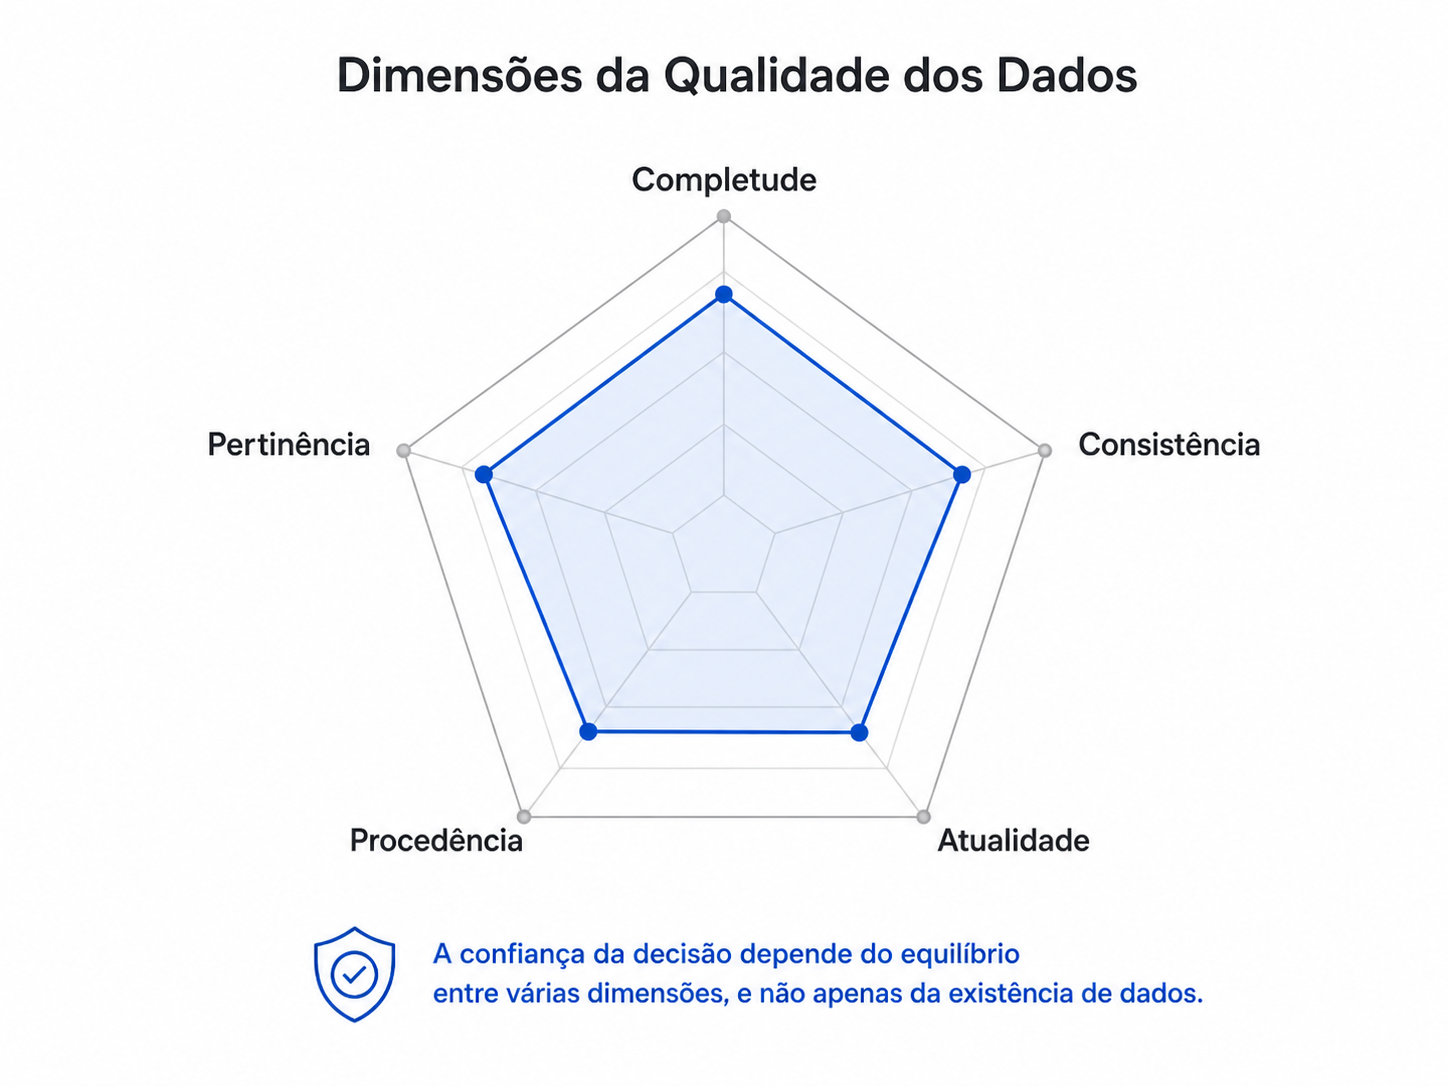
\includegraphics[width=0.5\linewidth]{img/dimensoesQualidadeDados.png}
    \caption{Radar da qualidade dos dados}
    \label{fig:qualidade-dados}
\end{figure}

\subsection{Adaptação ao contexto}

A adaptação ao contexto é outra característica essencial dos sistemas de automação inteligente. Diferentemente de sistemas baseados exclusivamente em regras fixas, sistemas inteligentes podem modificar sua resposta de acordo com variáveis ambientais, comportamentais e operacionais. Eles podem considerar horário, localização, perfil do usuário, histórico de ações, estado de sensores, nível de risco e regras específicas do domínio. Essa capacidade aumenta a utilidade da automação, mas também amplia a complexidade da validação da confiança.

No artigo \textit{Estudo da inteligência artificial aplicada em Internet das Coisas, voltada na automação residencial}, Welliton Sousa da Cunha \cite{cunha2018} mostra que a integração entre IA e IoT em automação residencial permite que sistemas aprendam comportamentos dos habitantes e adaptem rotinas conforme seus hábitos. Tal perspectiva é importante porque demonstra que a automação inteligente não deve ser vista apenas como execução de comandos, mas como interpretação contínua de contexto. Em uma residência inteligente, por exemplo, uma mesma ação pode ser adequada em determinado horário e inadequada em outro; pode ser segura para um usuário e arriscada para outro; pode ser esperada em uma situação comum e suspeita em uma situação excepcional.

A adaptação, entretanto, reduz a previsibilidade imediata do sistema. Quanto mais variáveis são consideradas, maior é a dificuldade de antecipar todas as combinações possíveis de entrada e saída. Esse ponto é central para o tema deste trabalho: sistemas adaptativos precisam de mecanismos de validação que verifiquem se a decisão é apropriada ao contexto específico em que será executada. Não basta que o sistema tenha aprendido um padrão; é necessário confirmar se o padrão ainda é válido, se o ambiente não mudou e se a ação não viola restrições operacionais.

Do ponto de vista algorítmico, a adaptação ao contexto pode ser tratada por meio de modelos de contexto, regras condicionais, sistemas de recomendação, técnicas de detecção de anomalias e classificadores probabilísticos. Esses mecanismos permitem estimar se uma ação é compatível com o comportamento esperado. No entanto, a decisão final deve considerar também critérios externos ao modelo, como limites de risco, normas de segurança, autorizações e necessidade de supervisão humana. Dessa forma, a validação da confiança deve combinar inferência estatística e regras de governança.

A adaptação ao contexto também exige que os sistemas lidem com incerteza. Em muitos casos, o ambiente não fornece todas as informações necessárias para uma decisão plenamente segura. Nesses cenários, o algoritmo de validação deve reconhecer a insuficiência informacional e reduzir o nível de autonomia da automação. Uma ação de baixo risco pode ser permitida mesmo com confiança moderada; uma ação crítica, por outro lado, deve ser bloqueada ou encaminhada para confirmação humana quando o contexto não for suficientemente claro.

\subsection{Segurança, controle e rastreabilidade}

A confiança em sistemas de automação inteligente depende também da capacidade de garantir segurança, controle e rastreabilidade. Uma decisão automatizada pode ser coerente do ponto de vista técnico e, ainda assim, não ser legítima se o sistema não tiver autorização para executá-la. Por isso, a validação da confiança deve verificar não apenas a qualidade da inferência, mas também a legitimidade da ação. Essa legitimidade envolve permissões, identidade, trilhas de auditoria, integridade da comunicação e possibilidade de responsabilização posterior.

No artigo \textit{Decentralized IoT Permission Management using NFTs: Implementation and Evaluation on Low-Cost Blockchains}, Pedro F. F. Abreu, Maria R. F. M. Ferreira, Geraldo A. Sarmento Neto, Thiago A. R. da Silva, Glauber D. Gonçalves, Ricardo A. L. Rabelo e José V. dos Reis Junior \cite{abreu2025} contribuem para esse debate ao apresentar uma abordagem em que permissões podem ser vinculadas a dispositivos e verificadas por meio de mecanismos descentralizados. Ainda que o uso de blockchain e NFTs não seja uma solução universal para todos os sistemas de automação, o trabalho demonstra a importância de tratar permissões como elementos verificáveis, auditáveis e resistentes a alterações indevidas. Para a validação da confiança, isso significa que uma ação automatizada só deve ser aceita quando houver prova suficiente de autorização.

Além da autorização formal, é necessário considerar riscos internos e comportamentos aparentemente legítimos. No artigo \textit{Smart Insiders: Exploring the Threat from Insiders using the Internet-of-Things}, Jason R. C. Nurse, Arnau Erola, Ioannis Agrafiotis, Michael Goldsmith e Sadie Creese \cite{nurse2015} analisam como dispositivos de IoT podem ampliar a superfície de ataque relacionada a ameaças internas em organizações. Os autores chamam atenção para o fato de que dispositivos conectados, inclusive pessoais, podem introduzir novos vetores de ataque em ambientes corporativos. Essa perspectiva é relevante porque demonstra que a confiança não pode se basear apenas na identidade declarada do usuário ou do dispositivo. É preciso avaliar comportamento, contexto, frequência, histórico e indícios de uso indevido.

Em sistemas de automação inteligente, segurança e controle devem operar em múltiplas camadas. A primeira camada envolve autenticação, isto é, a verificação de quem ou o que está interagindo com o sistema. A segunda envolve autorização, relacionada ao que essa entidade pode fazer. A terceira envolve integridade, garantindo que dados e comandos não foram adulterados. A quarta envolve auditoria, permitindo reconstruir a cadeia de eventos que levou a determinada decisão. A quinta envolve contenção, impedindo que uma ação de alto risco seja executada sem validação adicional.

A rastreabilidade é especialmente importante porque permite que a confiança seja avaliada depois da execução da ação. Em sistemas inteligentes, nem sempre é possível antecipar todos os cenários de uso, mas é possível registrar entradas, saídas, justificativas, permissões e resultados. Esses registros permitem auditoria, correção de falhas, melhoria de modelos e responsabilização. Portanto, um algoritmo de validação da confiança deve produzir não apenas uma decisão binária de permitir ou negar, mas também evidências sobre os motivos que levaram a essa decisão.

\begin{figure}[htbp]
    \centering
    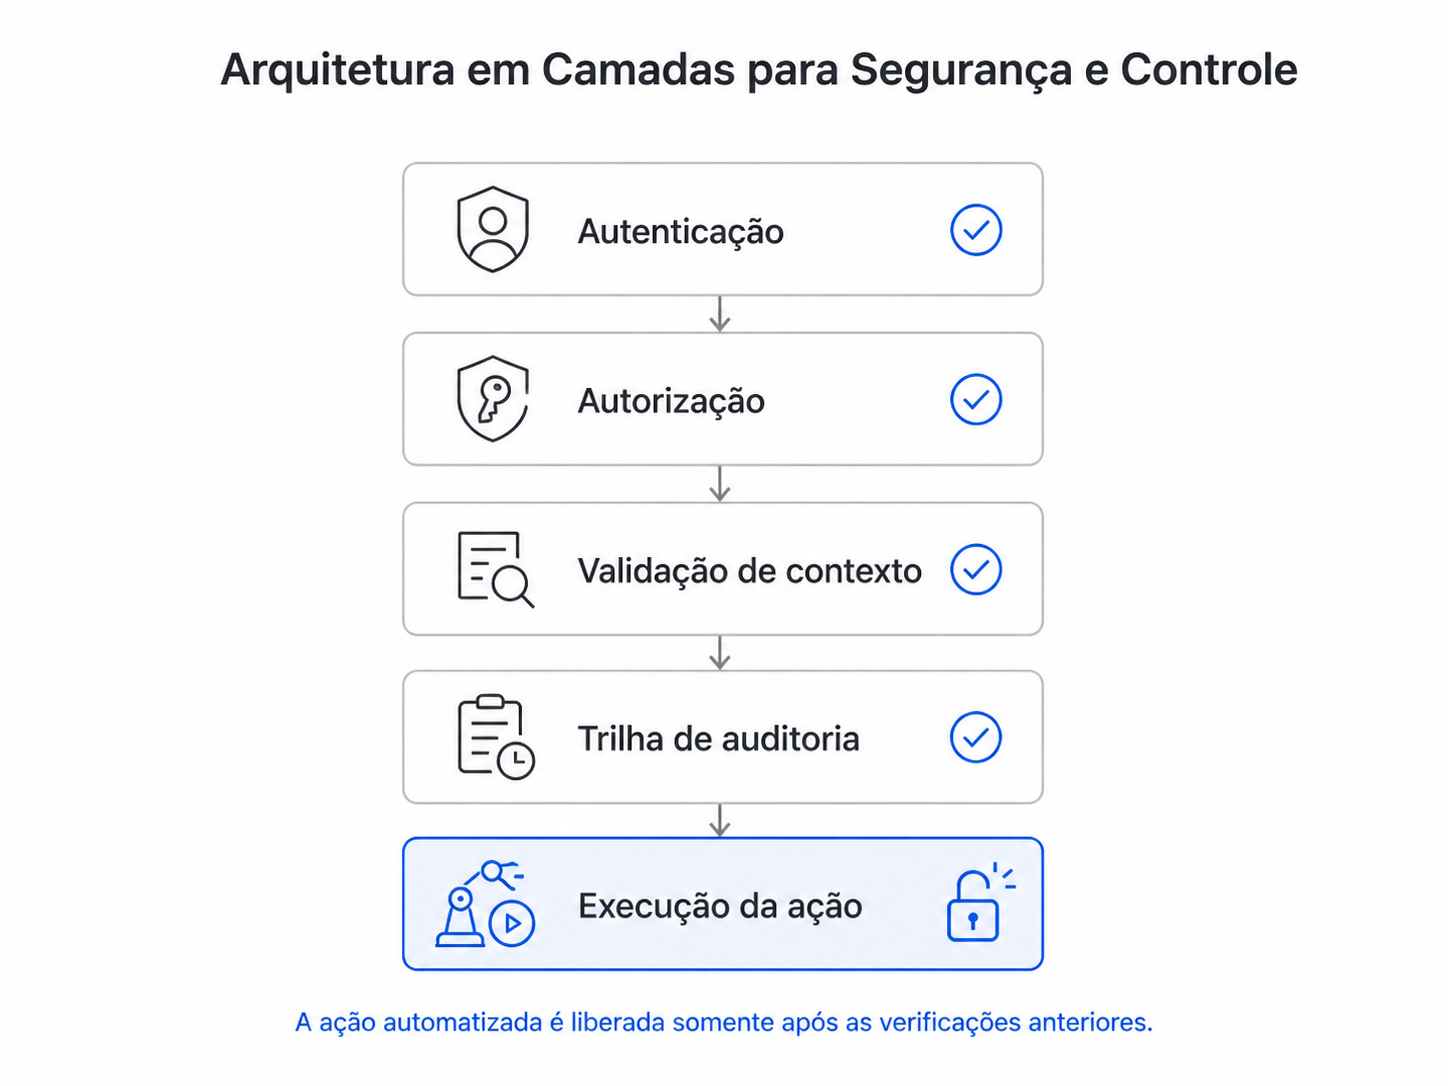
\includegraphics[width=0.5\linewidth]{img/arquiteturaCamadas.png}
    \caption{Arquitetura em Camadas}
    \label{fig:arquitetura-camadas}
\end{figure}

\subsection{Validação da confiança}

A validação da confiança é o ponto de convergência entre os conceitos discutidos anteriormente. Ela pode ser entendida como o processo pelo qual o sistema avalia se uma decisão automatizada possui condições suficientes para ser executada com segurança, coerência e legitimidade. Essa validação não se limita a medir a precisão do modelo, mas envolve a análise conjunta dos dados utilizados, do contexto observado, das permissões existentes, dos riscos associados e da possibilidade de auditoria.

Do ponto de vista computacional, um algoritmo de validação da confiança pode funcionar como uma camada decisória intermediária. Essa camada recebe a ação proposta pelo sistema inteligente e calcula um nível de confiança com base em diferentes critérios. Quando o nível de confiança é alto e o risco é baixo, a ação pode ser executada automaticamente. Quando o nível de confiança é intermediário ou o risco é relevante, o sistema pode solicitar confirmação humana. Quando o nível de confiança é baixo, a ação deve ser bloqueada ou encaminhada para análise. Assim, a validação da confiança transforma a automação em um processo controlado por limiares e evidências.

Esse processo pode ser organizado como uma avaliação progressiva das condições que sustentam a decisão automatizada. Em vez de depender de um único indicador, a validação deve observar um conjunto de dimensões complementares. Primeiro, verifica-se se os dados que alimentam o sistema são completos, consistentes, atuais e provenientes de fontes confiáveis. Em seguida, avalia-se se a inferência produzida pelo sistema é coerente com as regras do domínio e com o comportamento esperado para aquele tipo de situação. Depois, examina-se se o contexto permite a ação proposta, considerando usuário, ambiente, histórico, horário, sensibilidade da operação e possíveis exceções.

Além desses elementos, a validação precisa verificar se a entidade envolvida possui autorização legítima para executar a ação e se existem mecanismos suficientes de segurança, conformidade e rastreabilidade. Em sistemas críticos, por exemplo, uma decisão automatizada não deve ser aceita apenas porque parece tecnicamente correta; ela também precisa ser justificável, auditável e compatível com o impacto da ação. Em automações simples e reversíveis, o nível de exigência pode ser menor, mas ainda assim deve existir algum critério mínimo de controle. Dessa forma, a validação da confiança funciona como uma análise estruturada de evidências, e não como uma simples etapa final de confirmação.

Essa abordagem não deve ser interpretada como uma solução única ou definitiva. Em aplicações reais, cada dimensão pode ser avaliada por técnicas diferentes. A qualidade dos dados pode ser examinada por regras de consistência, completude e atualização. A confiança na inferência pode ser analisada por estabilidade da resposta, comparação com regras do domínio e identificação de incertezas. A adequação ao contexto pode ser verificada por regras de negócio e detecção de anomalias. A segurança pode depender de autenticação, autorização e análise de risco. A rastreabilidade pode ser observada pela existência de logs, justificativas e evidências de auditoria.

No artigo \textit{Erros, falhas e perturbações digitais em alucinações das IAs generativas: tipologia, premissas e epistemologia da comunicação}, André Lemos \cite{lemos2024} amplia essa discussão ao diferenciar erros, falhas e perturbações digitais. Essa distinção é útil porque ajuda a compreender que nem toda decisão inadequada possui a mesma origem. Um erro pode decorrer de uma inferência logicamente incorreta ou de uma resposta incompatível com uma regra esperada. Uma falha pode estar associada a problemas técnicos externos, como indisponibilidade de serviço, defeito de sensor ou perda de conectividade. Uma perturbação, por sua vez, pode emergir da interação entre sistema, usuários, ambiente e valores sociais, produzindo efeitos indesejados mesmo quando o sistema opera dentro de sua lógica formal.

Aplicada à automação inteligente, essa distinção indica que a validação da confiança deve ser capaz de identificar diferentes tipos de risco. Se a decisão decorre de dados ruins, o problema está na cadeia informacional. Se decorre de uma inferência incerta, o problema está no modelo ou no algoritmo. Se decorre de uso indevido por agente autorizado, o problema está na camada de segurança e comportamento. Se decorre de impacto social ou operacional imprevisto, o problema está na relação entre sistema e contexto. Portanto, validar confiança exige uma abordagem híbrida, que combine critérios técnicos e sociotécnicos.

A validação da confiança também deve ser proporcional ao impacto da ação. Nem toda automação exige o mesmo grau de verificação. Ações reversíveis, de baixo custo e baixo risco podem ser executadas com menor rigor. Ações irreversíveis, sensíveis ou potencialmente danosas devem exigir maior nível de confiança, maior rastreabilidade e, em muitos casos, intervenção humana. Essa proporcionalidade evita dois problemas: a automação excessivamente permissiva, que aceita riscos indevidos, e a automação excessivamente restritiva, que perde utilidade por bloquear ações simples.


\subsection{Síntese das dimensões de validação}

A partir dos autores analisados, é possível sintetizar que a confiança em sistemas de automação inteligente depende da articulação entre dados, modelos, contexto, permissões, segurança e auditoria. No artigo \textit{Trust Management in the Internet of Things: A Survey}, Ferrag, Maglaras e Janicke \cite{ferrag2019} contribuem para a compreensão do gerenciamento de confiança em ambientes IoT heterogêneos. No artigo \textit{Descoberta de conhecimento em base de dados de eventos de desligamentos de empresas de distribuição}, Tronchoni, Pretto, Rosa e Lemos \cite{tronchoni2010} evidenciam a necessidade de qualificação dos dados antes da aplicação de técnicas de inteligência artificial. No artigo \textit{Estudo da inteligência artificial aplicada em Internet das Coisas, voltada na automação residencial}, Cunha \cite{cunha2018} demonstra a importância da adaptação ao contexto em sistemas de automação baseados em IA e IoT. No artigo \textit{Decentralized IoT Permission Management using NFTs: Implementation and Evaluation on Low-Cost Blockchains}, Abreu et al. \cite{abreu2025} reforçam a dimensão verificável das permissões em IoT. No artigo \textit{Smart Insiders: Exploring the Threat from Insiders using the Internet-of-Things}, Nurse et al. \cite{nurse2015} destacam riscos internos e novos vetores de ataque em ambientes conectados. Por fim, no artigo \textit{Erros, falhas e perturbações digitais em alucinações das IAs generativas: tipologia, premissas e epistemologia da comunicação}, Lemos \cite{lemos2024} amplia a análise ao diferenciar erro, falha e perturbação em sistemas digitais.

A Tabela \ref{tab:dimensoes-confianca} apresenta uma síntese das dimensões teóricas que podem orientar a construção ou análise de algoritmos de validação da confiança.

\begin{table}[ht]
\centering
\caption{Dimensões para validação da confiança em sistemas de automação inteligente}
\label{tab:dimensoes-confianca}
\begin{tabular}{|p{3.2cm}|p{5.0cm}|p{5.0cm}|}
\hline
\textbf{Dimensão} & \textbf{Pergunta de validação} & \textbf{Implicação algorítmica} \\
\hline
Qualidade dos dados & Os dados são completos, consistentes, atuais e adequados à decisão? & Aplicar checagens de consistência, normalização, validação de origem e detecção de anomalias. \\
\hline
Confiança da inferência & O modelo produziu uma resposta estável, coerente e suficientemente segura? & Utilizar métricas de confiança, incerteza, margem de decisão e comparação com regras do domínio. \\
\hline
Adequação ao contexto & A ação faz sentido para o usuário, ambiente, horário, histórico e situação observada? & Combinar regras contextuais, perfis de uso, histórico de comportamento e análise de exceções. \\
\hline
Segurança e permissão & A entidade possui autorização legítima para executar a ação proposta? & Verificar autenticação, autorização, integridade, reputação e possíveis sinais de abuso. \\
\hline
Rastreabilidade & A decisão pode ser explicada, auditada e reconstruída posteriormente? & Registrar entradas, justificativas, permissões, resultados, logs e evidências de execução. \\
\hline
Proporcionalidade do risco & O nível de autonomia concedido é compatível com o impacto da ação? & Definir limiares para executar, solicitar confirmação humana ou bloquear a ação. \\
\hline
\end{tabular}
\end{table}

Com base nessa síntese, o presente trabalho considera que algoritmos de validação da confiança devem atuar como mecanismos de governança da automação inteligente. Eles devem impedir que a autonomia do sistema seja exercida sem critérios verificáveis e, ao mesmo tempo, permitir que ações seguras sejam executadas com eficiência. Assim, a validação da confiança não é apenas uma etapa técnica adicional, mas um requisito para que sistemas de automação inteligente possam ser adotados de forma responsável, transparente e auditável.




\section{Trabalhos Relacionados}

Esta seção apresenta os trabalhos relacionados ao tema \textit{Algoritmos de validação da confiança em sistemas de automação inteligente}. A análise foi organizada a partir de seis artigos selecionados no levantamento bibliográfico, considerando quatro aspectos principais: a estratégia adotada por cada trabalho, suas vantagens, suas limitações e sua relação com o problema motivador deste artigo. Em conjunto, os estudos mostram que a confiança em automações inteligentes não depende de um único mecanismo, mas de uma combinação entre qualidade dos dados, controle de acesso, segurança, rastreabilidade, interpretação de erros e adequação ao contexto de uso.

\subsection{Gerenciamento de confiança em Internet das Coisas}

Ferrag, Maglaras e Janicke \cite{ferrag2019} apresentam um levantamento sobre gerenciamento de confiança em ambientes de Internet das Coisas. A estratégia do artigo consiste em organizar e comparar modelos de confiança aplicáveis a redes compostas por dispositivos heterogêneos, considerando abordagens baseadas em reputação, autenticação, criptografia, aprendizado de máquina e mecanismos de segurança distribuída. O foco central está em compreender como uma entidade pode avaliar se outra entidade, como sensor, serviço, usuário ou dispositivo, deve ser considerada confiável em determinado contexto de interação.

A principal vantagem desse trabalho é oferecer uma visão ampla das técnicas existentes para construção de confiança em IoT. Essa visão é importante porque sistemas de automação inteligente normalmente dependem de múltiplos componentes conectados, e uma decisão automatizada pode ser comprometida caso qualquer elemento da cadeia apresente comportamento malicioso, instável ou não autorizado. Como desvantagem, por se tratar de um estudo de levantamento, o artigo não propõe um algoritmo único e pronto para aplicação direta em um domínio específico. Além disso, muitos modelos de confiança discutidos na literatura dependem de premissas difíceis de garantir em ambientes reais, como disponibilidade contínua de dados, padronização entre dispositivos e capacidade computacional suficiente.

A associação com o problema motivador é direta, pois o presente artigo busca investigar algoritmos de validação da confiança em sistemas de automação inteligente. O trabalho de Ferrag, Maglaras e Janicke contribui ao demonstrar que a confiança pode ser modelada como uma propriedade calculável, dinâmica e dependente de contexto. Assim, ele fornece uma base conceitual para pensar mecanismos de validação que atribuem níveis de confiança antes da execução de ações automatizadas.

\subsection{Ameaças internas em ambientes IoT}

Nurse et al. \cite{nurse2015} analisam a ameaça de usuários internos em ambientes de Internet das Coisas. A estratégia do artigo é deslocar o foco tradicional da segurança, geralmente concentrado em ataques externos, para o risco de dispositivos pessoais e inteligentes serem utilizados por insiders maliciosos ou descuidados dentro de organizações. Os autores discutem vetores de ataque relacionados a dispositivos vestíveis, objetos conectados, coleta indevida de dados, vazamento de informações e dificuldade de detecção em ambientes nos quais os perímetros de segurança se tornam menos definidos.

A vantagem do trabalho está em ampliar a compreensão da confiança para além da autenticação formal. Um usuário ou dispositivo pode estar autorizado a acessar determinado ambiente e, ainda assim, agir de modo incompatível com a confiança esperada. Essa perspectiva é relevante para automações inteligentes porque tais sistemas não devem validar apenas se uma entidade possui credenciais, mas também se seu comportamento, contexto e finalidade são compatíveis com a ação solicitada. Como desvantagem, o artigo tem caráter exploratório e apresenta uma agenda de pesquisa, sem implementar um mecanismo de detecção ou validação aplicável diretamente.

A relação com o problema motivador está na necessidade de validar confiança considerando riscos internos. Em sistemas de automação inteligente, uma ação automatizada pode ser tecnicamente correta, mas insegura se for acionada por um agente comprometido, por um dispositivo desconhecido ou por uma situação anômala. Portanto, o trabalho reforça que algoritmos de validação da confiança devem considerar comportamento, histórico, origem da solicitação e sensibilidade da operação.

\subsection{Gerenciamento descentralizado de permissões com NFTs}

Abreu et al. \cite{abreu2025} propõem um modelo descentralizado de gerenciamento de permissões para IoT utilizando \textit{Non-Fungible Tokens} e contratos inteligentes. A estratégia consiste em representar dispositivos como ativos digitais únicos e utilizar contratos inteligentes para registrar, delegar e revogar permissões de acesso. A solução foi avaliada em plataformas de baixo custo, como Polygon, Arbitrum e Optimism, com foco em custo de transação e consumo de gás.

A principal vantagem da proposta é tornar o controle de acesso mais auditável, transparente e resistente a falhas de autoridade central. Como os registros de permissão ficam associados a contratos inteligentes, torna-se possível verificar quem possui acesso, por quanto tempo e em quais condições. Isso contribui para a rastreabilidade, uma dimensão essencial da confiança em automações inteligentes. Outra vantagem é a análise de viabilidade econômica, pois sistemas IoT podem envolver grande quantidade de dispositivos e operações frequentes. Como desvantagem, a solução depende de infraestrutura blockchain, conectividade, integração com dispositivos reais e tratamento de latência. Além disso, o modelo ainda precisa avançar em políticas mais expressivas, como regras contextuais, atributos dinâmicos e integração com cenários físicos complexos.

A associação com o problema motivador ocorre pela dimensão de permissão verificável. Em sistemas de automação inteligente, não basta que uma decisão seja logicamente adequada; é necessário comprovar que a entidade responsável possui autorização para executá-la. O trabalho contribui ao mostrar uma estratégia técnica para validar confiança por meio de identidade, delegação, revogação e auditoria de permissões.

\subsection{Inteligência artificial e IoT na automação residencial}

Cunha \cite{cunha2018} investiga a aplicação de inteligência artificial em Internet das Coisas voltada à automação residencial. A estratégia do artigo é discutir a evolução da automação residencial tradicional para a domótica inteligente, na qual sensores, atuadores e algoritmos de aprendizagem são utilizados para adaptar o ambiente aos hábitos dos moradores. O trabalho destaca o uso de árvores de decisão, especialmente o algoritmo C4.5, como mecanismo de aprendizado a partir dos dados coletados.

A vantagem desse estudo é demonstrar de forma aplicada como a automação deixa de ser apenas uma sequência de regras fixas e passa a envolver percepção, aprendizagem e adaptação. Essa abordagem aproxima a discussão de contextos reais de uso, nos quais conforto, economia, segurança e personalização dependem da capacidade do sistema de interpretar padrões de comportamento. Como desvantagem, o trabalho discute a automação residencial em nível mais conceitual e não aprofunda mecanismos formais para validação da confiança das decisões geradas pelo sistema. Também há desafios relacionados à privacidade dos dados dos moradores, à qualidade das leituras dos sensores e à segurança dos dispositivos conectados.

A relação com o problema motivador aparece porque a domótica inteligente exemplifica um ambiente no qual decisões automatizadas afetam diretamente pessoas e espaços físicos. Se o sistema aprende hábitos incorretamente, utiliza dados incompletos ou executa ações sem considerar exceções, a confiança do usuário pode ser comprometida. Assim, o artigo reforça a necessidade de algoritmos que validem os dados, o contexto e o risco antes da execução de ações automatizadas.

\subsection{Qualificação de dados e Redes Bayesianas em sistemas de distribuição}

Tronchoni et al. \cite{tronchoni2010} exploram a técnica de Descoberta de Conhecimento em Bases de Dados para qualificar informações de eventos de desligamento em empresas de distribuição de energia. A estratégia adotada é transformar dados brutos, subjetivos e inconsistentes, coletados por equipes de campo, em uma base mais adequada para o treinamento de uma Rede Bayesiana. O objetivo é apoiar o diagnóstico de causas de desligamentos forçados e orientar decisões de operação, manutenção e investimento.

A principal vantagem do trabalho está em evidenciar que a confiabilidade de um sistema inteligente depende fortemente da qualidade dos dados usados como entrada. A Rede Bayesiana só se torna útil após um processo de seleção, limpeza, transformação e validação das informações disponíveis. Esse ponto é essencial para automações inteligentes, pois algoritmos de decisão podem parecer sofisticados, mas produzir resultados frágeis quando alimentados por dados incompletos, ambíguos ou mal classificados. Como desvantagem, a metodologia depende de um processo prévio de preparação dos dados e de conhecimento do domínio para estruturar variáveis relevantes. Além disso, Redes Bayesianas podem ter dificuldade de manutenção quando o domínio muda rapidamente ou quando novas variáveis precisam ser incorporadas.

A associação com o problema motivador está na dimensão de validação informacional. Um algoritmo de confiança precisa verificar se a decisão automatizada está apoiada em dados consistentes e suficientes. O artigo mostra que, antes de confiar no resultado produzido pela inteligência artificial, é necessário confiar no processo de qualificação da informação que alimenta o modelo.

\subsection{Erros, falhas e perturbações em inteligências artificiais generativas}

Lemos \cite{lemos2024} analisa erros, falhas e perturbações digitais a partir do fenômeno das alucinações em inteligências artificiais generativas. A estratégia do artigo é propor uma distinção conceitual entre erro, falha e perturbação, mostrando que eventos disruptivos em sistemas digitais não devem ser observados apenas como defeitos técnicos isolados, mas como manifestações que revelam características internas dos objetos digitais e de suas relações sociotécnicas.

A vantagem desse trabalho é oferecer uma lente crítica para compreender decisões inadequadas produzidas por sistemas inteligentes. Em automações baseadas em IA, uma resposta incorreta pode decorrer de erro lógico do modelo, falha externa de infraestrutura, dado inadequado ou perturbação produzida pela interação entre sistema, usuário e contexto social. Essa distinção ajuda a evitar diagnósticos simplistas e contribui para a criação de mecanismos de validação mais completos. Como desvantagem, o artigo possui abordagem predominantemente teórica e comunicacional, sem propor métricas ou algoritmos específicos para detecção automática desses eventos.

A relação com o problema motivador é relevante porque algoritmos de validação da confiança precisam diferenciar tipos de risco. Uma automação não deve apenas bloquear resultados incorretos; ela deve identificar por que uma decisão parece não confiável e qual resposta é proporcional ao problema detectado. Nesse sentido, o trabalho de Lemos contribui para a formulação de critérios que separem erro de inferência, falha operacional e perturbação contextual.

\subsection{Síntese dos trabalhos analisados}

Os trabalhos relacionados mostram que a validação da confiança em sistemas de automação inteligente exige uma abordagem integrada. Ferrag, Maglaras e Janicke \cite{ferrag2019} contribuem com modelos de confiança para IoT; Nurse et al. \cite{nurse2015} evidenciam riscos internos e comportamentais; Abreu et al. \cite{abreu2025} apresentam mecanismos verificáveis de permissão e auditoria; Cunha \cite{cunha2018} demonstra a adaptação de sistemas inteligentes a ambientes residenciais; Tronchoni et al. \cite{tronchoni2010} reforçam a importância da qualificação dos dados; e Lemos \cite{lemos2024} amplia a análise dos erros e falhas em sistemas inteligentes.

A partir dessa comparação, observa-se que nenhum dos trabalhos, isoladamente, resolve todo o problema da confiança em automações inteligentes. Entretanto, cada um contribui com uma dimensão necessária: confiança entre entidades, segurança contra abuso, autorização verificável, adaptação contextual, qualidade informacional e análise de falhas. Portanto, o presente artigo se associa a esses estudos ao defender que algoritmos de validação da confiança devem combinar diferentes evidências antes de permitir que uma automação execute ações com impacto real.


\section{Metodologia}

Este trabalho será desenvolvido por meio de uma pesquisa aplicada, de natureza qualitativa e caráter exploratório. A pesquisa é considerada aplicada porque busca organizar uma proposta de validação da confiança voltada a sistemas de automação inteligente, com possibilidade de uso futuro em cenários práticos. O caráter qualitativo decorre da análise conceitual das dimensões de confiança, risco, segurança, permissão, rastreabilidade e qualidade dos dados. Já o caráter exploratório está relacionado à investigação de estratégias ainda em consolidação na literatura, especialmente quando aplicadas à validação de ações sugeridas ou executadas por sistemas inteligentes.

Quanto aos procedimentos, a pesquisa combina revisão bibliográfica, análise comparativa dos trabalhos relacionados e proposição de um fluxo metodológico para validação da confiança. A revisão bibliográfica tem a função de identificar os principais conceitos e critérios utilizados em estudos sobre automação inteligente, Internet das Coisas, segurança, permissões, qualidade dos dados e falhas em sistemas baseados em inteligência artificial. A etapa propositiva organiza esses critérios em um processo de validação que poderá ser testado futuramente por meio de cenários simulados, estudos de caso ou protótipos computacionais.

\subsection{Procedimento metodológico da pesquisa}

A primeira etapa da metodologia consiste na definição do tema e do problema de pesquisa. Em seguida, são estabelecidas palavras-chave e critérios de busca para localizar trabalhos relacionados ao tema. Após o levantamento bibliográfico inicial, os artigos encontrados são registrados e avaliados quanto à aderência ao problema investigado. Os trabalhos aderentes passam por extração das principais contribuições, classificação por dimensão de análise e verificação de sua utilidade para a construção da proposta. Os trabalhos não aderentes são descartados ou mantidos apenas como apoio complementar.

Esse processo permite refinar progressivamente a base teórica do estudo, evitando que a proposta seja construída apenas a partir de exemplos isolados. A Figura \ref{fig:metodologia-pesquisa} apresenta o fluxo utilizado para organizar o levantamento, a coleta, a filtragem e a síntese dos trabalhos empregados no projeto.

\begin{figure}[htbp]
    \centering
    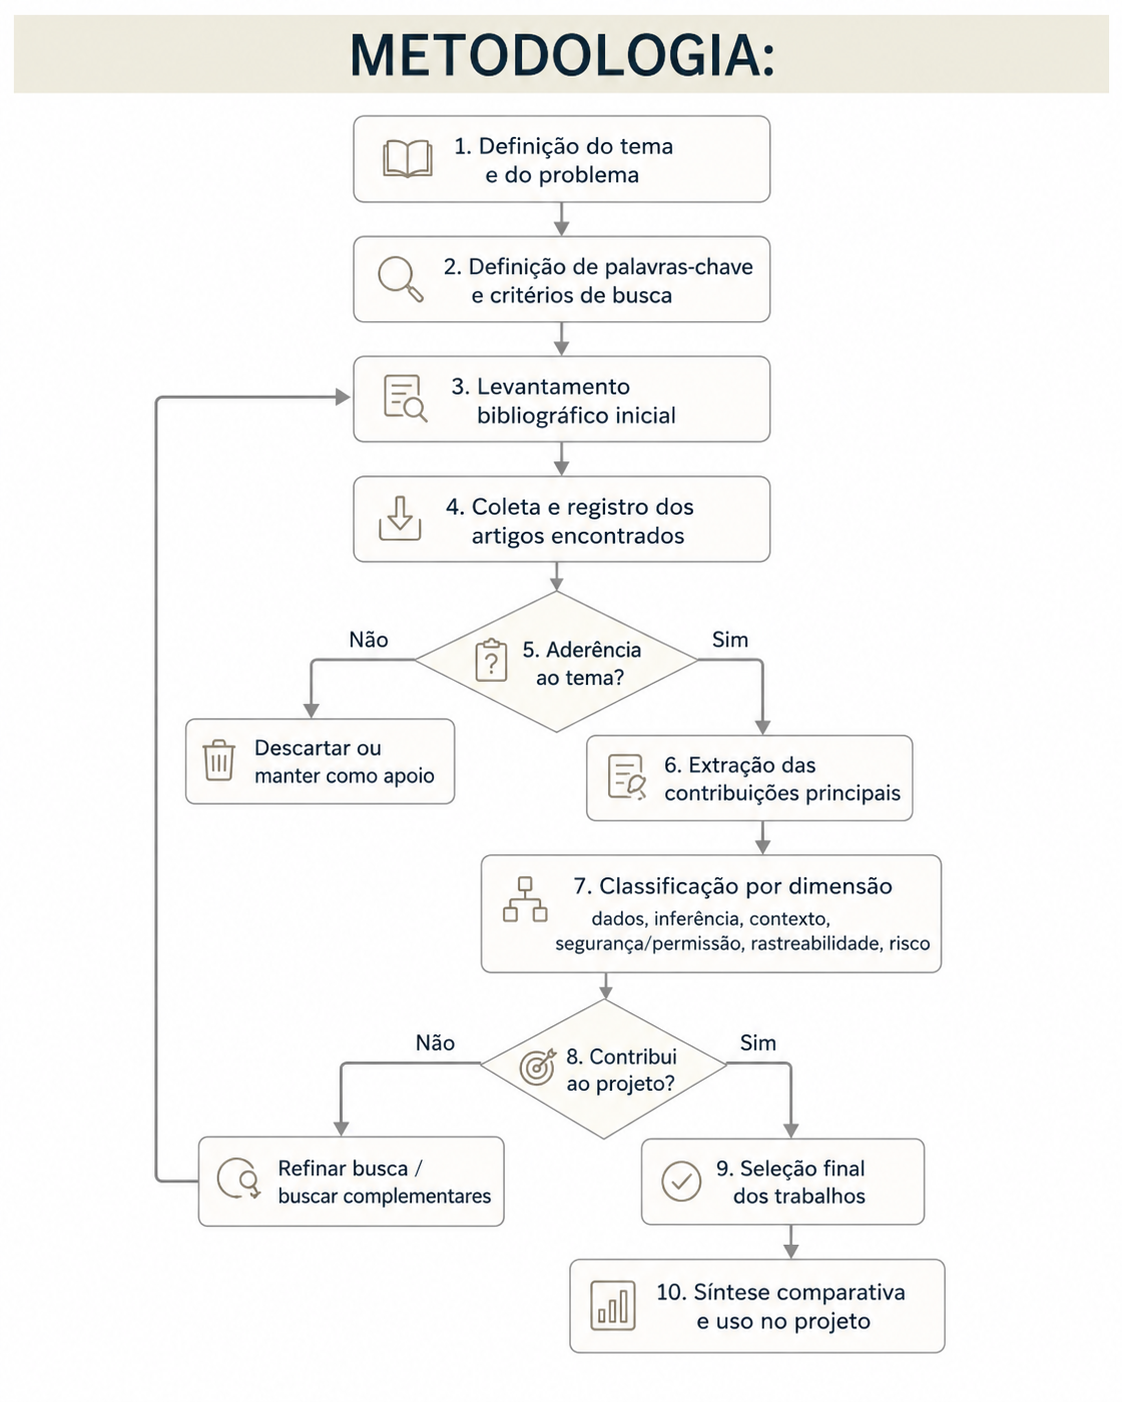
\includegraphics[width=0.62\linewidth]{img/metodologia.png}
    \caption{Fluxo metodológico de levantamento, coleta e seleção dos trabalhos}
    \label{fig:metodologia-pesquisa}
\end{figure}

\subsection{Metodologia da proposta}

A estratégia proposta parte do princípio de que uma automação inteligente não deve executar uma ação apenas porque ela foi sugerida por um modelo ou agente. Antes da execução, a ação proposta deve ser submetida a uma camada de validação responsável por reunir evidências, calcular um nível de confiança, estimar o risco e definir a resposta mais adequada. Essa resposta pode ser a execução automática, a solicitação de confirmação humana ou o bloqueio da ação para análise posterior.

O processo inicia com o recebimento da ação proposta, contendo entrada de dados, contexto e comando sugerido pela automação. Em seguida, ocorre a coleta de evidências, incluindo dados disponíveis, histórico de uso, origem da informação, permissões associadas e condições contextuais. A validação da confiança é realizada por dimensões, considerando qualidade dos dados, coerência da inferência, adequação ao contexto, segurança, permissão e rastreabilidade. A partir dessas dimensões, o sistema calcula um nível de confiança e um nível de risco para apoiar a decisão.

Quando a confiança é suficiente e o risco é aceitável, a ação pode ser executada. Quando o resultado é intermediário ou envolve operação sensível, o sistema solicita confirmação humana. Quando a confiança é baixa ou o risco é elevado, a ação deve ser bloqueada ou encaminhada para análise. Em todos os casos, o resultado da decisão deve ser registrado para permitir auditoria, explicação posterior e melhoria contínua dos critérios de validação. A Figura \ref{fig:metodologia-proposta} resume essa estratégia.

\begin{figure}[htbp]
    \centering
    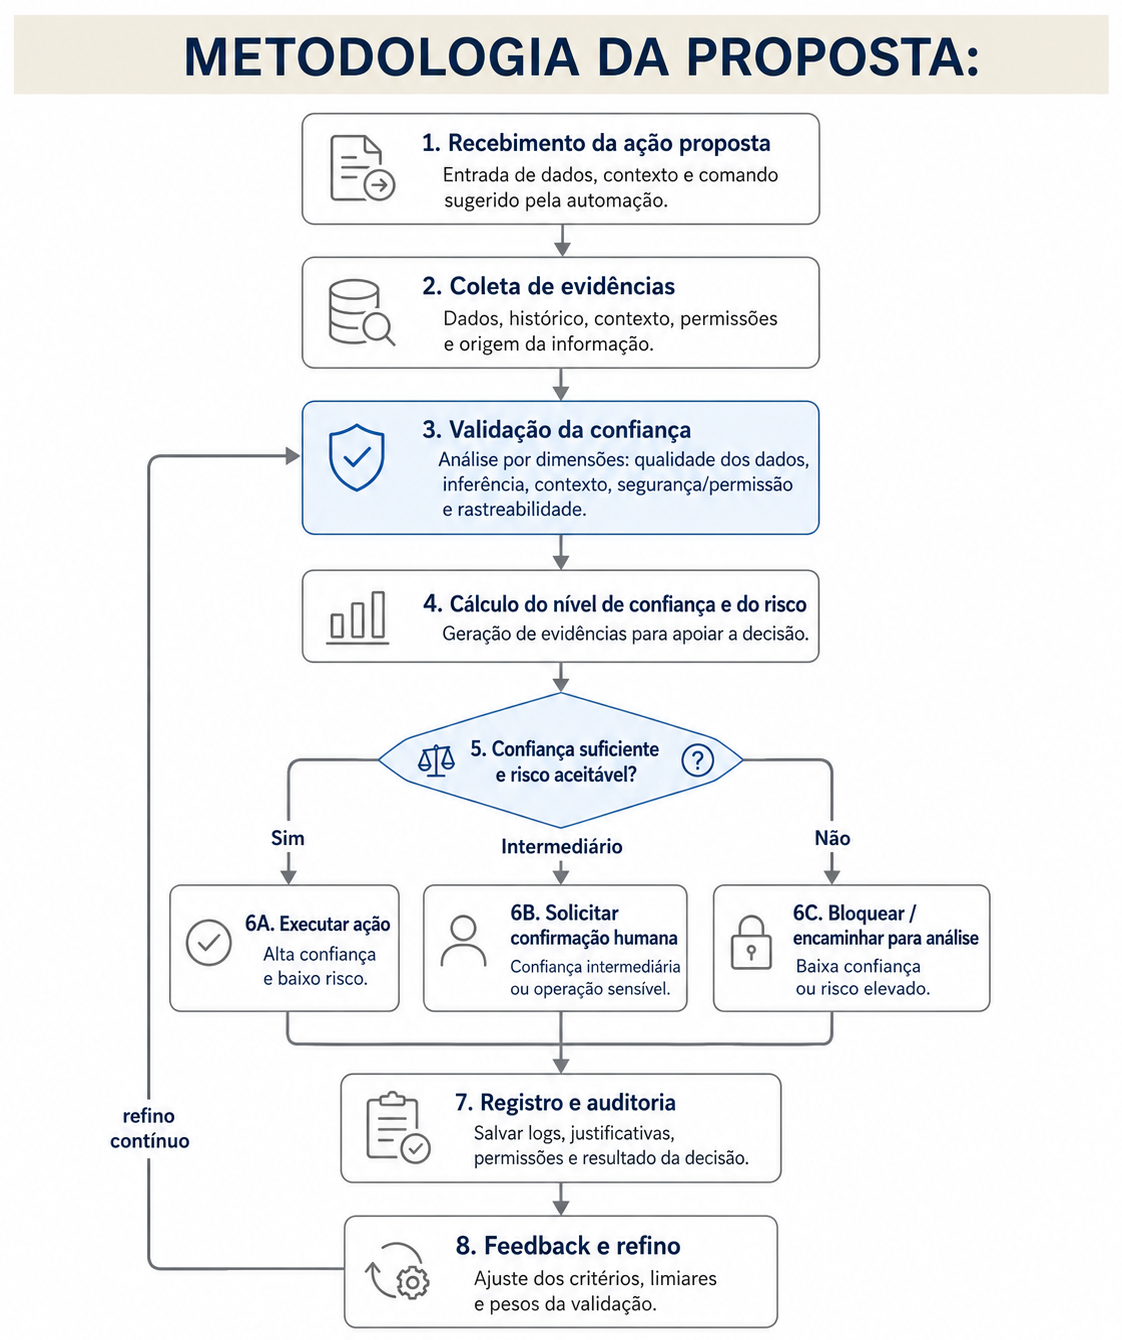
\includegraphics[width=0.64\linewidth]{img/metodologiaProposta.png}
    \caption{Metodologia da proposta para validação da confiança em automações inteligentes}
    \label{fig:metodologia-proposta}
\end{figure}

Na etapa de teste futuro, a proposta poderá ser avaliada por meio de cenários controlados. Esses cenários devem representar ações automatizadas com diferentes níveis de risco, como ações simples e reversíveis, ações com dados incompletos, ações sem permissão adequada e ações sensíveis que exigem validação humana. Para cada cenário, deverão ser observados os critérios utilizados pelo algoritmo, o nível de confiança calculado, a decisão final tomada e a justificativa registrada. Dessa forma, será possível verificar se a metodologia contribui para tornar a automação mais segura, auditável e proporcional ao risco da operação.

\subsection{Cronograma esperado}

O cronograma da pesquisa foi organizado em seis etapas principais, distribuídas ao longo de seis meses. As primeiras etapas concentram-se na consolidação teórica e no refinamento dos critérios de análise. As etapas seguintes envolvem a modelagem da proposta, a preparação de cenários de avaliação, a análise dos resultados esperados e a redação final do artigo.

\begin{table}[htbp]
\centering
\caption{Cronograma esperado da pesquisa}
\label{tab:cronograma-pesquisa}
\footnotesize
\resizebox{\textwidth}{!}{%
\begin{tabular}{|p{6.0cm}|c|c|c|c|c|c|}
\hline
\textbf{Etapa} & \textbf{Mês 1} & \textbf{Mês 2} & \textbf{Mês 3} & \textbf{Mês 4} & \textbf{Mês 5} & \textbf{Mês 6} \\
\hline
Definição do problema, objetivos e delimitação do escopo & X &  &  &  &  &  \\
\hline
Levantamento bibliográfico e seleção dos trabalhos relacionados & X & X &  &  &  &  \\
\hline
Extração das contribuições e classificação por dimensões de confiança &  & X & X &  &  &  \\
\hline
Modelagem da metodologia de validação da confiança e dos critérios de risco &  &  & X & X &  &  \\
\hline
Definição de cenários para teste futuro da proposta &  &  &  & X & X &  \\
\hline
Análise, ajustes, redação final e revisão da formatação no modelo SBC &  &  &  &  & X & X \\
\hline
\end{tabular}%
}
\end{table}

Esse cronograma funciona como uma previsão inicial de execução. Caso a proposta avance para implementação ou validação empírica, novas etapas poderão ser acrescentadas, como construção de protótipo, execução de experimentos, coleta de métricas quantitativas e comparação com abordagens existentes.



\section{Resultados esperados}

Como resultado esperado, a metodologia proposta deve organizar um processo de validação capaz de apoiar decisões de automações inteligentes antes da execução de ações sensíveis. Por se tratar de uma proposta metodológica, os resultados são apresentados como expectativas de aplicação e por meio de cenários sintéticos. A expectativa central é que o sistema não execute automaticamente toda ação sugerida por um modelo inteligente, mas avalie previamente evidências de qualidade dos dados, contexto, permissão, rastreabilidade e risco.

Espera-se que a camada de validação produza três respostas principais: execução automática, confirmação humana ou bloqueio da ação. A execução automática deve ocorrer em ações simples, reversíveis e bem fundamentadas. A confirmação humana deve ser solicitada quando a confiança for intermediária ou quando o impacto da ação exigir supervisão. O bloqueio deve ocorrer em situações de baixa confiança, ausência de permissão, inconsistência de dados ou risco elevado.

\subsection{Exemplos sintéticos de aplicação}

A Tabela \ref{tab:resultados-esperados} apresenta exemplos sintéticos de aplicação da metodologia. Os percentuais são ilustrativos e indicam como diferentes evidências podem influenciar a classificação final da confiança. Em uma implementação real, esses valores poderiam ser calculados por regras ponderadas, modelos probabilísticos, classificadores supervisionados ou combinação de métricas de segurança, contexto, qualidade dos dados e histórico.

\begin{table}[!htbp]
\centering
\caption{Exemplos sintéticos de resultados esperados da metodologia proposta}
\label{tab:resultados-esperados}
\footnotesize
\resizebox{\textwidth}{!}{%
\begin{tabular}{|p{3.0cm}|p{4.3cm}|p{2.3cm}|p{2.5cm}|p{4.2cm}|}
\hline
\textbf{Cenário} & \textbf{Evidências avaliadas} & \textbf{Confiança esperada} & \textbf{Resposta esperada} & \textbf{Justificativa} \\
\hline
Automação residencial sugere desligar luzes externas durante o dia & Sensor de luminosidade ativo, horário compatível, histórico recorrente e ação reversível & Alta, acima de 85\% & Executar automaticamente & Ação de baixo risco, contexto coerente e simples reversão. \\
\hline
Sistema recomenda liberar dispositivo IoT desconhecido à rede interna & Dispositivo sem histórico, origem não validada e permissão não registrada & Baixa, abaixo de 50\% & Bloquear a ação & A falta de identidade confiável e permissão verificável aumenta o risco de acesso indevido. \\
\hline
Agente inteligente sugere enviar relatório gerado por IA a um cliente & Dados parcialmente verificados, conteúdo plausível e presença de informações sensíveis & Intermediária, entre 60\% e 80\% & Solicitar confirmação humana & A comunicação externa exige revisão para evitar erro, exposição indevida ou alucinação. \\
\hline
Automação operacional propõe desligar equipamento após leitura anômala de sensor & Sensor indica falha, mas há divergência com leituras de outros dispositivos & Intermediária ou baixa & Solicitar confirmação ou bloquear & A inconsistência entre fontes exige validação adicional antes de ação física relevante. \\
\hline
Sistema financeiro tenta aprovar pagamento fora do padrão histórico & Valor elevado, horário incomum e usuário com permissão limitada & Baixa & Bloquear e registrar alerta & O risco operacional e a incompatibilidade com o comportamento esperado justificam bloqueio preventivo. \\
\hline
\end{tabular}%
}
\end{table}

Os exemplos indicam que a confiança não deve ser analisada como medida única. Uma ação pode ser logicamente coerente, mas rejeitada por falta de permissão. De modo semelhante, uma ação pode partir de usuário autorizado e ainda assim ser insegura se os dados forem inconsistentes, o horário for incomum ou o impacto for elevado. Assim, o resultado esperado da metodologia é combinar diferentes dimensões de validação, em vez de depender exclusivamente da resposta produzida pelo modelo inteligente.

\subsection{Discussão dos resultados esperados}

A principal expectativa é que a metodologia funcione como uma camada de governança entre a inferência do sistema inteligente e a execução da ação automatizada. Essa camada não substitui os modelos de inteligência artificial, os controles de acesso ou os mecanismos de segurança existentes. Sua função é integrar essas informações em um processo decisório transparente, proporcional ao risco e passível de auditoria.

Em ambientes baseados em Internet das Coisas, a proposta pode contribuir para avaliar confiança entre dispositivos, usuários e serviços, conforme discutido por Ferrag, Maglaras e Janicke \cite{ferrag2019}. Em cenários com risco de uso indevido por usuários internos ou dispositivos autorizados, a metodologia reforça a análise de comportamento, contexto e histórico, aspecto relacionado às preocupações apresentadas por Nurse et al. \cite{nurse2015}. Quando a confiança depende de permissões verificáveis, a proposta se aproxima da discussão sobre rastreabilidade e delegação de acesso apresentada por Abreu et al. \cite{abreu2025}.

Outro resultado esperado é a melhoria da qualidade das decisões automatizadas por meio da validação dos dados de entrada. Conforme discutido por Tronchoni et al. \cite{tronchoni2010}, sistemas inteligentes dependem da qualidade das informações utilizadas no processo decisório. Portanto, quando os dados forem incompletos, contraditórios ou pouco confiáveis, a metodologia deve reduzir o grau de autonomia concedido à automação.

Também se espera que a proposta ajude a diferenciar tipos de falhas. Uma resposta inadequada pode decorrer de erro de inferência, falha de infraestrutura, inconsistência informacional, ausência de permissão ou perturbação contextual. Essa distinção é relevante porque a reação do sistema deve ser proporcional ao problema identificado, dialogando com a discussão de Lemos \cite{lemos2024} sobre erros, falhas e perturbações em sistemas digitais.

A proposta possui limitações. Os pesos atribuídos a cada dimensão de confiança podem variar conforme o domínio de aplicação, pois sistemas residenciais, financeiros, corporativos e infraestruturas críticas apresentam riscos distintos. Além disso, a metodologia depende de registros confiáveis, como logs, histórico, permissões e dados contextuais. Ainda assim, espera-se que ela contribua para reduzir a execução automática de ações inadequadas e aumentar a capacidade de auditoria quando falhas ocorrerem.

\section{Conclusão}

Este trabalho apresentou uma proposta de investigação sobre algoritmos de validação da confiança em sistemas de automação inteligente. A partir do referencial teórico e dos trabalhos relacionados, observou-se que a confiança não depende apenas da precisão de um modelo ou da capacidade de executar comandos automaticamente. Ela envolve qualidade dos dados, coerência da inferência, adequação ao contexto, segurança, permissão, rastreabilidade e proporcionalidade do risco.

A metodologia proposta organiza essas dimensões em um fluxo de validação anterior à execução da ação automatizada. Nesse fluxo, a automação deve reunir evidências, avaliar o contexto, verificar permissões, estimar o nível de confiança, calcular o risco e definir a resposta adequada: executar automaticamente, solicitar confirmação humana ou bloquear a ação. Essa estrutura busca impedir que decisões sejam executadas apenas por terem sido sugeridas por um agente inteligente.

Os resultados esperados indicam que a aplicação da metodologia pode melhorar a governança de sistemas automatizados em cenários com impacto operacional, financeiro, informacional ou físico. Os exemplos sintéticos demonstram que a mesma ação pode receber tratamentos diferentes conforme as evidências disponíveis, o histórico, a permissão e o risco envolvido. Assim, a confiança deve ser dinâmica, contextual e auditável.

Como contribuição, o artigo apresenta uma organização conceitual que pode servir de base para protótipos, estudos de caso ou experimentos computacionais. Em trabalhos futuros, recomenda-se implementar a metodologia em ambiente controlado, definir métricas quantitativas para cada dimensão de confiança, testar diferentes formas de ponderação dos critérios e comparar a proposta com abordagens baseadas apenas em regras fixas ou apenas em modelos de inteligência artificial.

Conclui-se que a validação da confiança é requisito essencial para a adoção responsável de sistemas de automação inteligente. Quanto maior o grau de autonomia concedido a esses sistemas, maior deve ser a capacidade de verificar, justificar, limitar e auditar suas ações. Portanto, algoritmos de validação da confiança devem compor a arquitetura central de sistemas inteligentes seguros, transparentes e compatíveis com o uso real.

\bibliographystyle{sbc}
\bibliography{referencias}

\end{document}
